\begin{figure}[H]
    \centering
    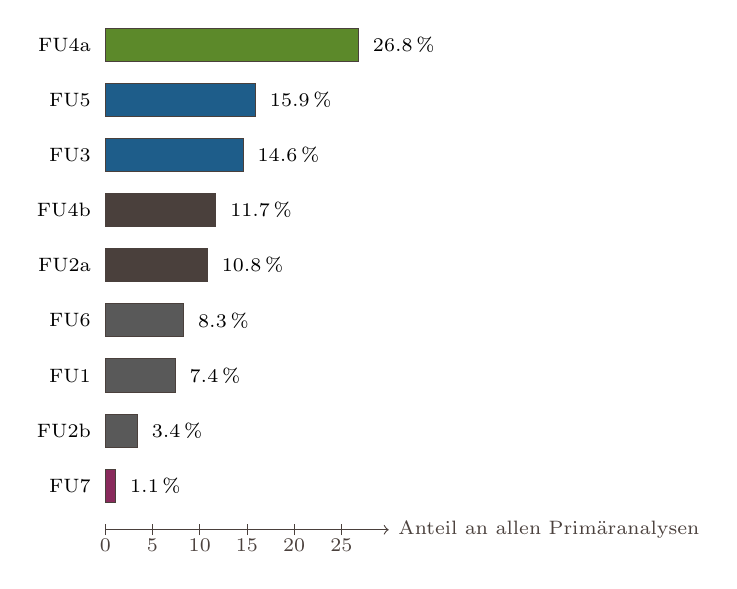
\begin{tikzpicture}[x=0.12cm, y=0.7cm]
        % CI-Farben
        \definecolor{ciPrimaryLine}{HTML}{1E5D8A}
        \definecolor{ciSecondaryLine}{HTML}{4A403C}
        \definecolor{ciAccent}{HTML}{89572A}
        \definecolor{ciBrightArea}{HTML}{B3B3B3}
        \definecolor{ciDepthArea}{HTML}{133855}
        \definecolor{ciPositive}{HTML}{5C892A}
        \definecolor{ciNegative}{HTML}{892A5C}
        \definecolor{ciNeutral}{HTML}{595959}
        \definecolor{ciStability}{HTML}{4A403C}
        \definecolor{ciGlint}{HTML}{E0E0E0}

        % Daten: Anteil in Prozent / Label / y-Position / CI-Farbe
        \foreach \p/\t/\y/\c in {
            26.8/FU4a/8/ciPositive,
            15.9/FU5/7/ciPrimaryLine,
            14.6/FU3/6/ciPrimaryLine,
            11.7/FU4b/5/ciSecondaryLine,
            10.8/FU2a/4/ciSecondaryLine,
            8.3/FU6/3/ciNeutral,
            7.4/FU1/2/ciNeutral,
            3.4/FU2b/1/ciNeutral,
            1.1/FU7/0/ciNegative}
        {
            % Balken
            \draw[fill=\c, draw=ciStability, line width=0.3pt]
                (0,\y-0.3) rectangle (\p,\y+0.3);
            % FU-Label links
            \node[anchor=east, font=\scriptsize] at (-0.5,\y) {\t};
            % Prozent rechts
            \node[anchor=west, font=\scriptsize] at (\p+0.5,\y) {\pgfmathprintnumber[fixed,precision=1]{\p}\,\%};
        }

        % Achse
        \draw[->, ciStability, line width=0.4pt] (0,-0.8) -- (30,-0.8)
            node[anchor=west, font=\scriptsize] {Anteil an allen Primäranalysen};
        \foreach \x in {0,5,10,15,20,25}
            \draw[ciStability, line width=0.3pt] (\x,-0.9) -- (\x,-0.7)
                node[anchor=north, font=\scriptsize, yshift=-2pt] {\x};
	    \end{tikzpicture}
        \captionsetup{justification=justified,singlelinecheck=false}
        \caption{Verteilung der Analysen erster Ordnung auf die Forschungsunterfragen FU1–FU7}
        \caption*{\footnotesize Dargestellt ist der prozentuale Anteil der insgesamt 786 Primäranalysen je Forschungsunterfrage; die horizontale Balken-Darstellung sind absteigend nach Anteil sortiert, die Achse unten zeigt die Prozentwerte in 5-\%-Schritten.}
        \label{fig:primaranalysen-verteilung}
	\end{figure}
